\documentclass{exam}
\renewcommand{\thequestion}{Q.\arabic{question}}%
\usepackage[margin=1in]{geometry}
\usepackage{amsmath,amsfonts,amssymb}
\usepackage{multicol}
\usepackage{graphicx}
%\usepackage{nopageno}

\begin{document}


\begin{center}
\begin{minipage}{0.1\textwidth}

\includegraphics[scale=0.1]{vcet-logo.jpeg}
\end{minipage}
 \hfill 
\begin{minipage}{0.85\textwidth}
 \textbf{\Large \textbf{\begin{center}  Vidyavardhini's College of Engineering and Technology, Vasai (West) \end{center} }}
\end{minipage}

\vspace{0.3cm}
\textbf{\large \underline{First Year Engineering}} \\
\vspace{0.3cm}
\textbf{\large Academic Year: 2024-2025} \\
\vspace{0.3cm}
\textbf{\large Solution to the prevous year questions papers [2017 $-$ 2024] \footnote{This document has been compiled solely for the benefit of students. Permission is granted to use and distribute this material strictly for non-commercial purposes. Some content has been referenced from various academic sources, and all rights remain with the original copyright holders.} }\\
\end{center}

\noindent
\textbf{Subject: BSC102/AP} \hfill { \textbf{Date: 20/11/2024} }\\
%\textbf{Max Marks: 10} \hfill { \textbf{Duration: 1 Hr} }\\
\hrule
\begin{center}
\textbf{\large Module-5: Quantum Physics } 
\end{center}
\hrule
\vspace{0.3cm}

\begin{center} \textbf{ \Large De Broglie's Hypothesis of Matter Wave} \end{center}

\begin{questions}

\question \textbf{ Explain De Broglie's hypothesis of matter waves and deduce the expression for wavelength. \hfil
[3 Marks] [May-2019, May-2023]  
\\ OR \\
What is e Broglie's hypothesis? Derive expression for De Broglie's wavelength. \hfil [4 Marks] [May-2022, May-2024 (3M)] 
\\ OR \\
State de' Broglie hypothesis and derive an expression for de' Broglie wavelength. Mention three properties of matter waves. \hfil [5 Marks] [Dec-2023]
\\ OR \\
State properties of matter waves. \hfil [3 Marks] [Nov-2018,  May-2023]
\\ OR \\
	What are matter Waves? State three properties of matter waves. \hfil [3 Marks] [Dec-2022]
}

\textbf{Ans:} Interference, diffraction requires wave nature for their explanation. In photo-electric effect Einstein visualized the incident light as a sort of particles which he called photons and accounted for the emission of electrons as due to the collision between these photons and electrons bound to the metal. During the collision, the photon transfers all its energy to the electrons which results in the emission of photo electrons. Here the behaviour of light is same as that of a particle.

Louis De Broglie put forward the dual behaviour in terms of hypothesis which states If the radiation behaves as particle under certain circumstances, then one can even expect that, entities which ordinarily behave as particles to exhibit properties attributed to only waves under appropriate circumstances. The concept that matter behaves like a wave was proposed by Louis de Broglie in 1924. It is also referred to as the de Broglie hypothesis of matter waves. On the other hand de Broglie hypothesis is the combination of wave nature and particle nature.

If  E is the energy of a photon of radiation havinf frequency $\rm \nu$ and the same energy can be written for a wave as follows
\begin{center}
Then its energy is $\rm E = h \nu $.  (wave nature)\\
It can also be represented as $\rm E = mc^2 $.  (particle nature)\\
$\rm \therefore \quad h \nu = mc^2$ \\
\end{center}
\begin{equation*}
\therefore mc^2 = h \nu \implies \frac{mc^2}{c} = \frac{h \nu}{c} = \frac{h \nu c} {\lambda} \implies \therefore \lambda = \frac{h}{p}
\end{equation*}
where $\rm \lambda$ = De Broglie wavelength and p = momentum associated with photon which travels in free space.

\newpage

\textbf{Properties of matter waves}
\begin{enumerate}
\item The wavelength of a matter wave is inversely related to its particles momentum. if the particle moves faster, then the wavekegth will be smaller and vice versa
\item If the particle is at rest , then the de Broglie wavelength is infinite. Such waves cannot be visualized.
\item Matter wave can be reflected, refracted, diffracted and undergo interference
\item The amplitude of the matter waves at a particular region and time depends on the probability of finding the particle at the same region and time.
\item The position and momentum of the material particles cannot be determined accurately
and simultaneously.
\item  Matter wave is independent of the charge of the particle
\end{enumerate}

\question \textbf{ For an electron passing through potential difference 'V', show that its wavelength is;  \\ $\lambda = \frac{12.26}{\sqrt(V)}  A^{\circ}$. \hfil [5 Marks] [Nov-2018]  
}

\textbf{Ans:} De Broglie wavelength for a matter wave is given by 
\begin{equation*}
\rm \lambda = \frac{h}{p} = \frac{h}{mv}; \quad where \lambda = De Broglie wavelength \qquad (1)
\end{equation*}

From eqn. (1) we find that, if the particles like electrons are accelerated to various velocities, we can produce waves of various wavelengths. Thus higher the electron velocity, smaller will be the de-Broglie wavelength. If velocity v is given to an electron by accelerating it through a potential difference V, then the work done is converted to kinetic energy of electron. Hence, we can write 

\begin{equation*}
\rm mv = \sqrt{2meV} \qquad (2)
\end{equation*}
Substituting eqn.(2) in eqn.(1) we get

\begin{equation*}
\rm \lambda = \frac{h}{\sqrt{2meV}} 
\end{equation*}

Substituting the the values of h = 6.625 x $10^{-34}$ J-sec, m = 1.6 x $10^{-19}$ C, e = = 9.1 x $10^{-31}$ Kg for electron we get $\lambda = \frac{12.26}{\sqrt{V}}  A^{\circ}$.

\question \textbf{ Calculate the de Broglie wavelength of alpha particles accelerating through a potential difference of 150 volts. Given mass of Alpha particle is 6.68 x $10^{-17}$ Kg. \hfil [3 Marks] [May-2019]}

\textbf{Ans:}
\begin{center}
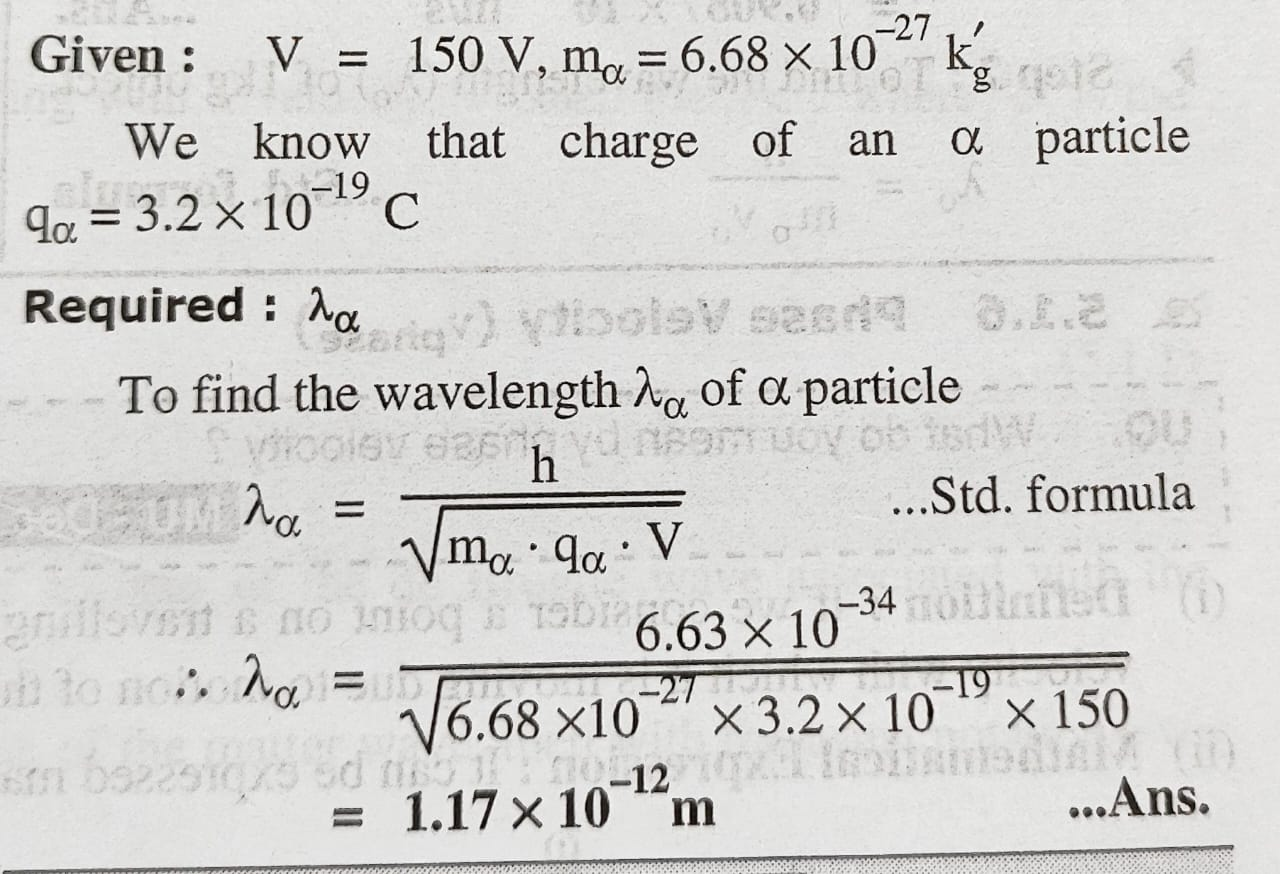
\includegraphics[scale=0.23]{Q3.jpeg}
\end{center}

\question \textbf{ What is the wavelength of a beam of neutron having: (i) an energy of 0.025 eV? (ii) an electron and photon each have wavelength of 2 $\rm A^{\circ}$. What are their momentum and enegy? $\rm m_{n} = 1.67 x 10^{-27} kg, h = 6.625 x 10^{-34}$ J-sec. \hfil  [5 Marks] [May-2017, Dec2021] }

\textbf{Ans:} Given Data: energy of neutron = 0.025 eV. \\ 
To find : wavelength of a beam. \\
Calculation :  \\

\begin{equation*} 
\rm  \lambda =  \frac{h}{\sqrt{2meV}} = \frac{6.626 x 10 ^{-34}}{ \sqrt{ 2 x 1.676 x 10 ^{-27} x 0.025 x 10^{-19} x 1.6 } }  =  1.8095 A^{\circ}
\end{equation*}
Hence wavelength is equal to 1.8095 $\rm A^{\circ}$ \\

2. Given Data $ \rm \lambda = 2 A^{\circ}, m_n = 1.676 x 10^{-27} kg, h= 6.625 x 10 ^{-34}  J-sec.$ \\

To find :- momentum and energy? \\
$\rm Calculations: \lambda = h/p \implies   p = 3.3125 x 10^{-24}$ kg-m/sec.

\begin{equation*}
\rm \lambda = h/\sqrt{2mE} \quad \implies \quad 2 x 10^{-10} = \frac{6.625 x 10^{-34}}{\sqrt{2 x 1.676 x 10^{-27} x E}} \quad \implies \quad E = 5.721 x 10^{-11} joules. 
\end{equation*}

 Hence momentum = 3.3125 x $10^{-24}$  kg-m/sec. and energy is = 5.721 x $10^{-11} $ joules.

\question \textbf{ Calculate the frequency and wavelength of photon whose energy is 75 eV. \\  \hfil [5 Marks] [May 2018] }

\question \textbf{ Find the de Broglie wavelength of (i) an electron accelerated through a potential difference of 182 Volts and (ii) 1 Kg object moving with a speed of 1 m/s. Comparing the results, explain why is the wave nature of matter not apparent in daily observations? \\ \hfil [5 Marks] [Dec-2022] } \\

\textbf{Ans:}
\begin{center}
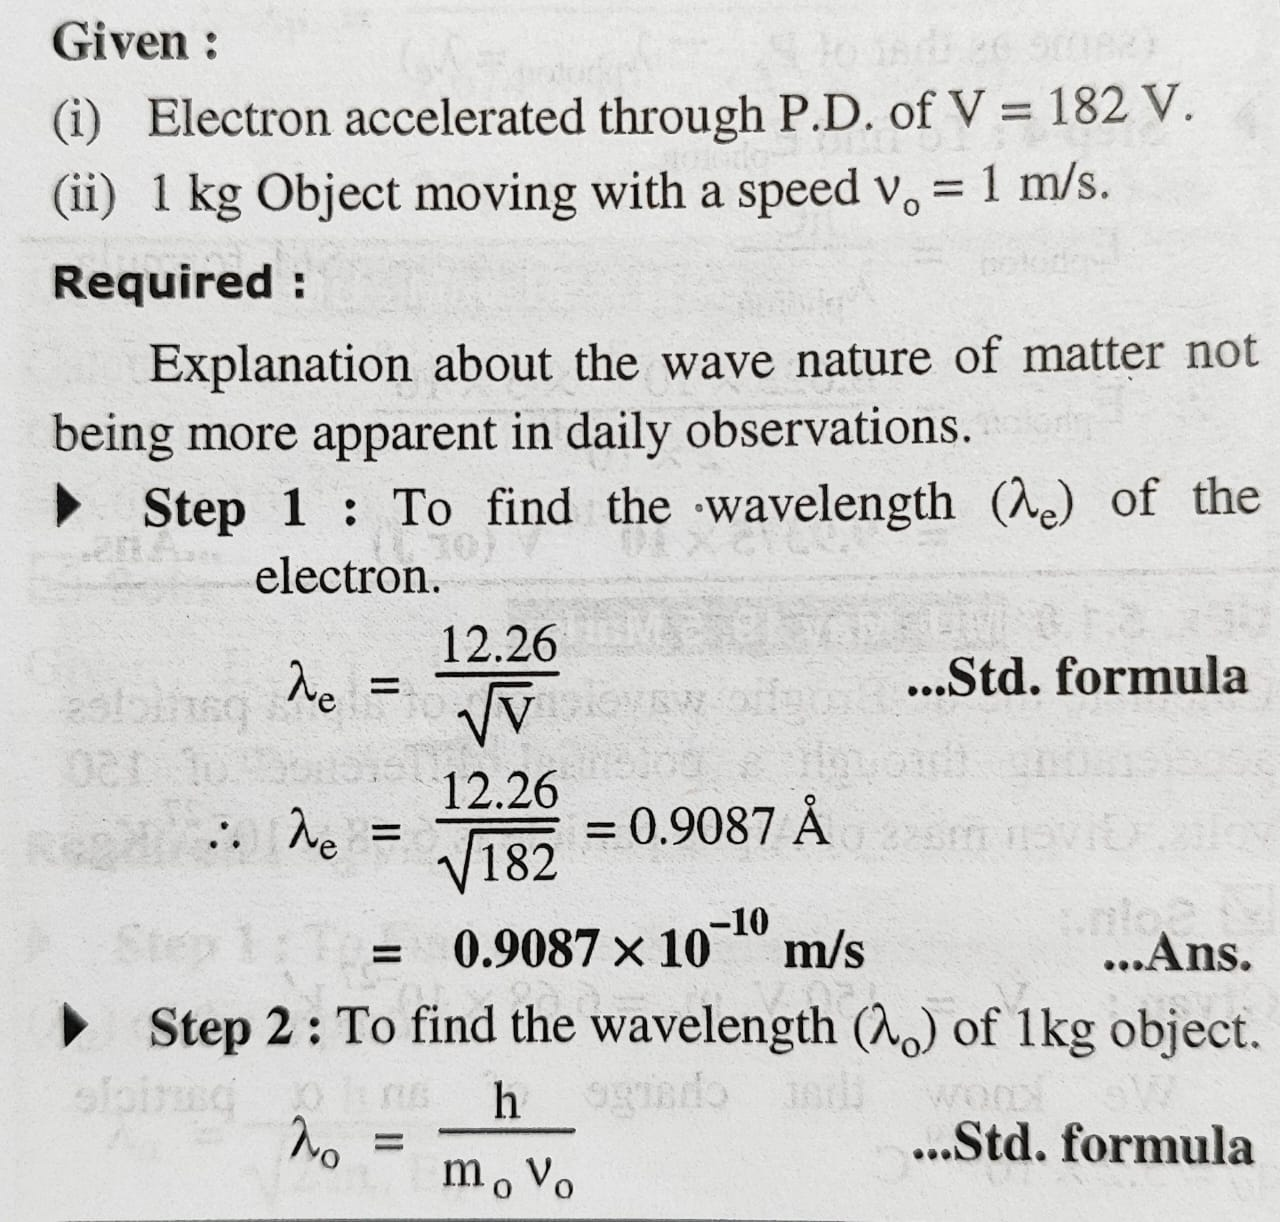
\includegraphics[scale=0.15]{Q5-1.jpeg}
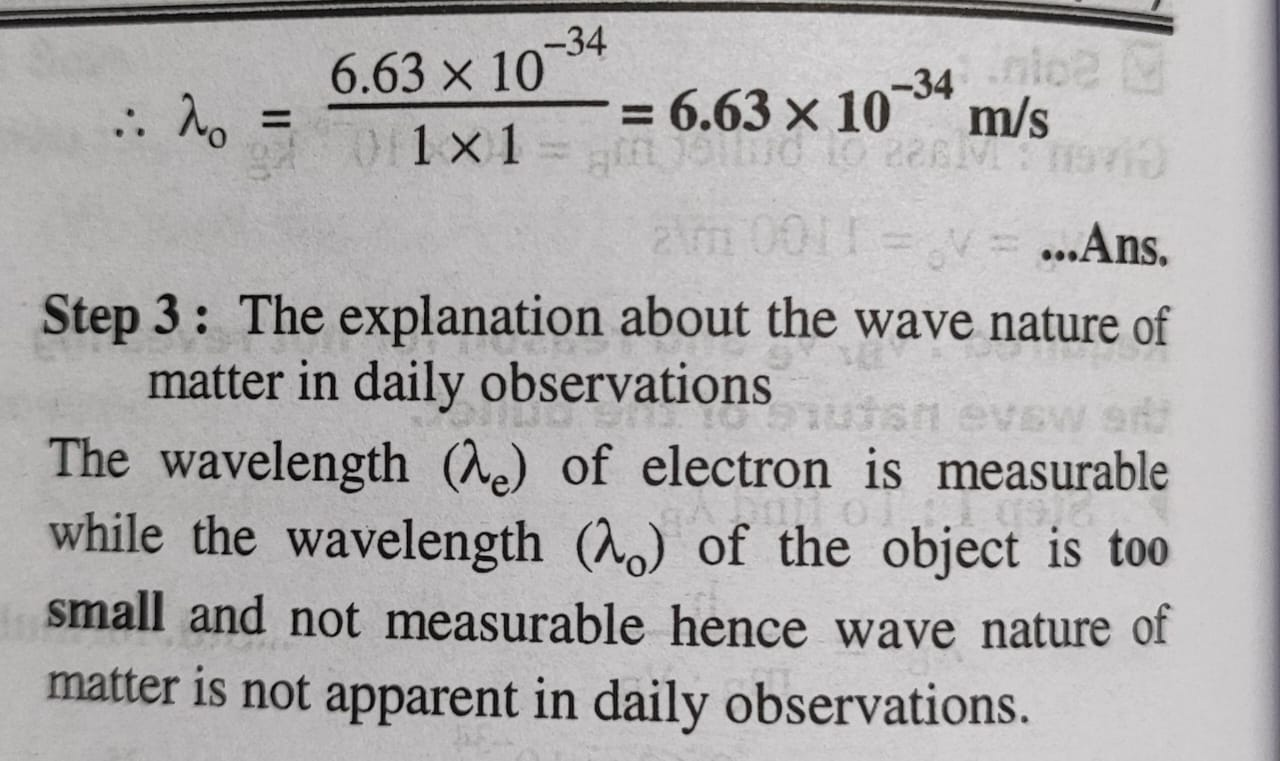
\includegraphics[scale=0.18]{Q5-2.jpeg}
\end{center}


\newpage

\begin{center} \textbf{ \Large Heisenberg's Uncertainty Principle} \end{center}

\question \textbf{ With Heisenberg's uncertainty principle prove that electron cannot survive in nucleus. An electron has a speed of 300 m/sec. with uncertainty of 0.01\%. Find the accuracy in its position. \hfil [4 Marks] [Dec-2017].
\\ OR \\
State Heisenberg's Uncertainty Principle. Show that electron doesn't exist in the nucleus. Find the accuracy in the position of an electron moving with speed 350 m/sec with uncertainty of 0.01\%. \hfil [8 Marks] [Nov-2018]  
\\ OR \\
Discuss Heisenberg's Uncertainty principle and prove that electrons cannot reside inside the nucleus of an atom using the same principle. \hfil [8 Marks] [May-2024] 
} 

\textbf{Ans:} Physical quantities like position, momentum, time, energy etc. can be measured accurately in macroscopic systems (i.e. classical mechanics). However, in the case of microscopic systems, the measurement of physical quantities for particles like electrons, protons, neutrons, photons etc are not accurate. If the measurement of one is certain and that of other will be uncertain. 

Thus according to uncertainty principle states that \textit{the position and the momentum of a particle in an atomic system cannot be determined simultaneously and accurately. If $\Delta$x is
the uncertainty associated with the position of a particle and $\Delta p_x$ the uncertainty associated with its momentum, then the product of these uncertainties will always be equal or greater than $h/4\pi$. That is} 
\begin{equation*}
\Delta x  \Delta p_x \geq h/4\pi 
\end{equation*}

\begin{center} \textbf{ Nonexistence of electron in the nucleus} \end{center}
	
The radius ‘r’ of the nucleus of any atom is of the order of $10^-14$m so that if an electron is confined in the nucleus, the uncertainty in its position will be of the order of 2r = $\Delta$x (say) i.e diameter of the nucleus. According to Heisenberg's Uncertainty principle 
\begin{equation*}
\Delta x  \Delta p_x \geq h/4\pi  \qquad \rm where \quad \Delta x \sim 10^{-14}  m
\end{equation*}
Therefore,
\begin{equation*}
\Delta p = h/(4 \pi \Delta x) = \rm 6.625 x 10^{-34}/ (4 \pi x 2x10^{-14}) = 2.63 x 10^{-21} kg-m/s
\end{equation*}
Taking $ \rm \Delta p \sim  p $ we can calculate energy using the formula

\begin{equation*}
\rm E^2 = c^2 [ p^2 + m_{0}^{2}c^2 ] = (3x 10^8)^2 x [(2.63 x 10-21)^2 + (9.1x10-31)^2 x (3x10^8)^2] 
\end{equation*}
\begin{equation*}
\rm = 7.932 x 10^{-13} J = 4957745 eV \sim 5 MeV
\end{equation*}

\textbf{However, the experimental investigations on beta decay reveal that the kinetic energies of electrons must be equal to 4MeV. Since there is a disagreement between theoretical and experimental energy values we can conclude that electrons cannot be found inside the nucleus.}

\question \textbf{ An electron has a speed of 400 m/sec with uncertainty of 0.01\%. Find the accuracy in its position. \hfil [5 Marks] [May-2023] }

\textbf{Ans:}
\begin{center}
	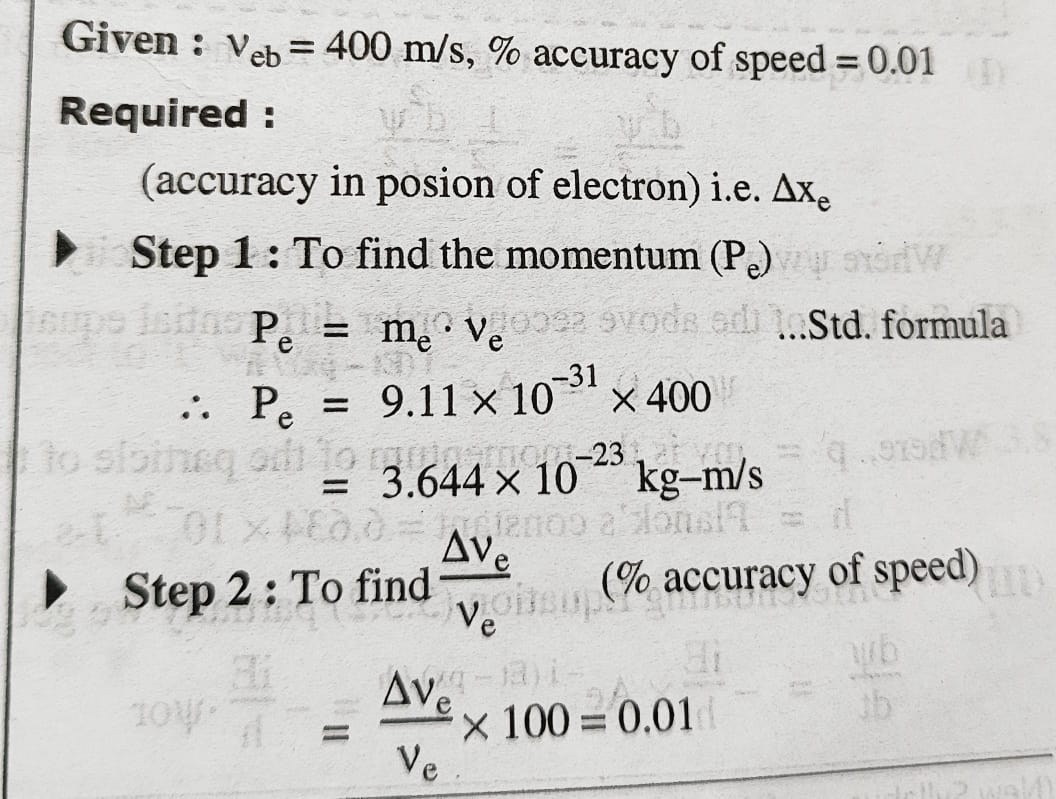
\includegraphics[scale=0.18]{Q10-1.jpeg}
	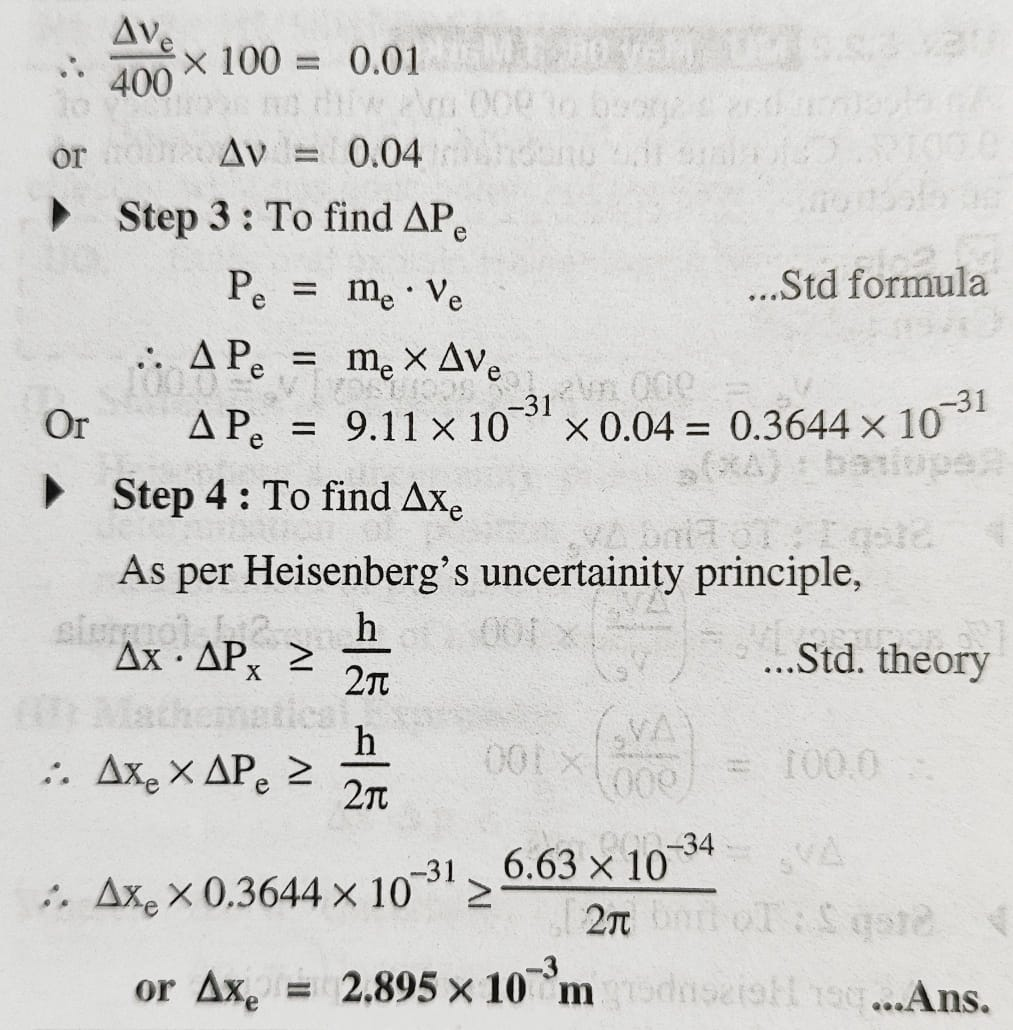
\includegraphics[scale=0.18]{Q10-2.jpeg}
\end{center}

\question \textbf{ Find the lowest energy of a neutron within a nucleus of dimension 10-14 m. given mass of a neutron $1.67 X 10^{-27}$ kg. \hfil [4 Marks] [May-2023] }

\textbf{Ans:}
\begin{center}
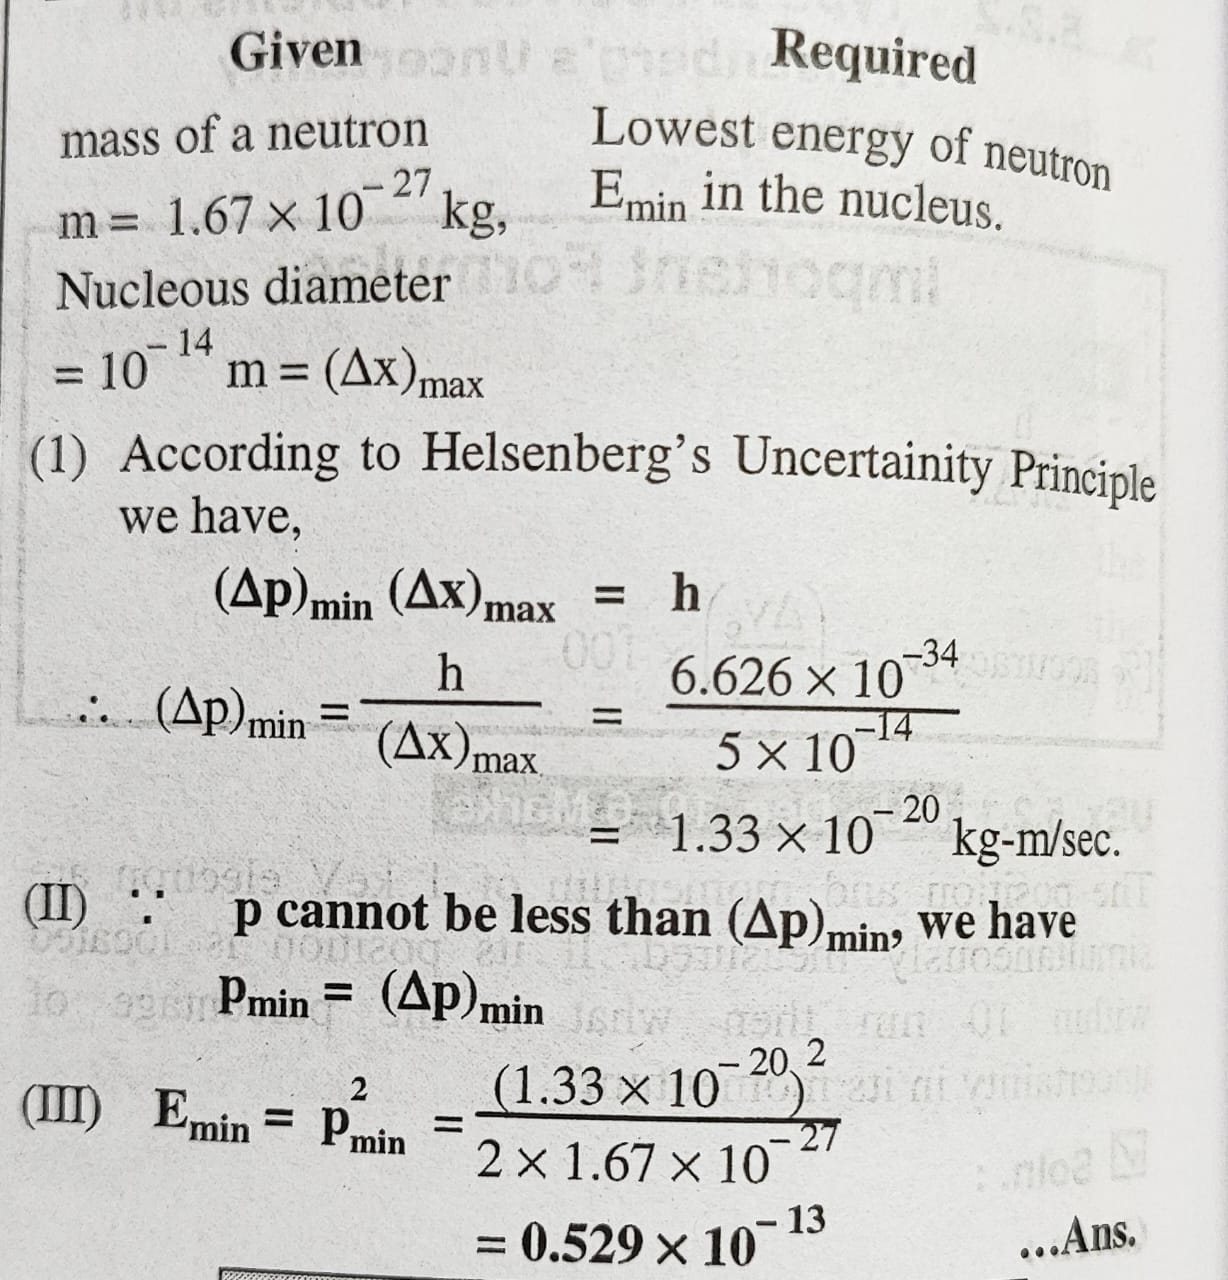
\includegraphics[scale=0.2]{Q11.jpeg}
\end{center}

	
\question \textbf{ Arrive at Heisenberg's uncertainty principle with single slit electron diffraction. An electron has a speed of 300m/sec. with uncertainty of 0.01\%. Find the accuracy in its position. \hfil [7 Marks] [May 2018] }

\textbf{Ans:} Similar to above problem(s)

\question \textbf{ Show that Non- Existence of electron in the Nucleus. Find the uncertainty in the position of electron. The speed of an to an accuracy of of 0.002\%. \hfil [8 Marks] [Dec-2019] }

\textbf{Ans:} Similar to above problem(s)
\newpage

\begin{center} \textbf{ \Large Schrödinger's Wave Equation} \end{center}


\question \textbf{ Derive Schrödinger's time dependent wave equation for matter waves. OR \\
Derive one dimensional Schrödinger's time dependent equation for matter waves. OR \\ Obtain one dimensional time dependent Schrödinger equation \\ \hfil [May-2017, 2018, 2023,  Dec-2022] [5 Marks]}

\textbf{Ans:}
\begin{center}
	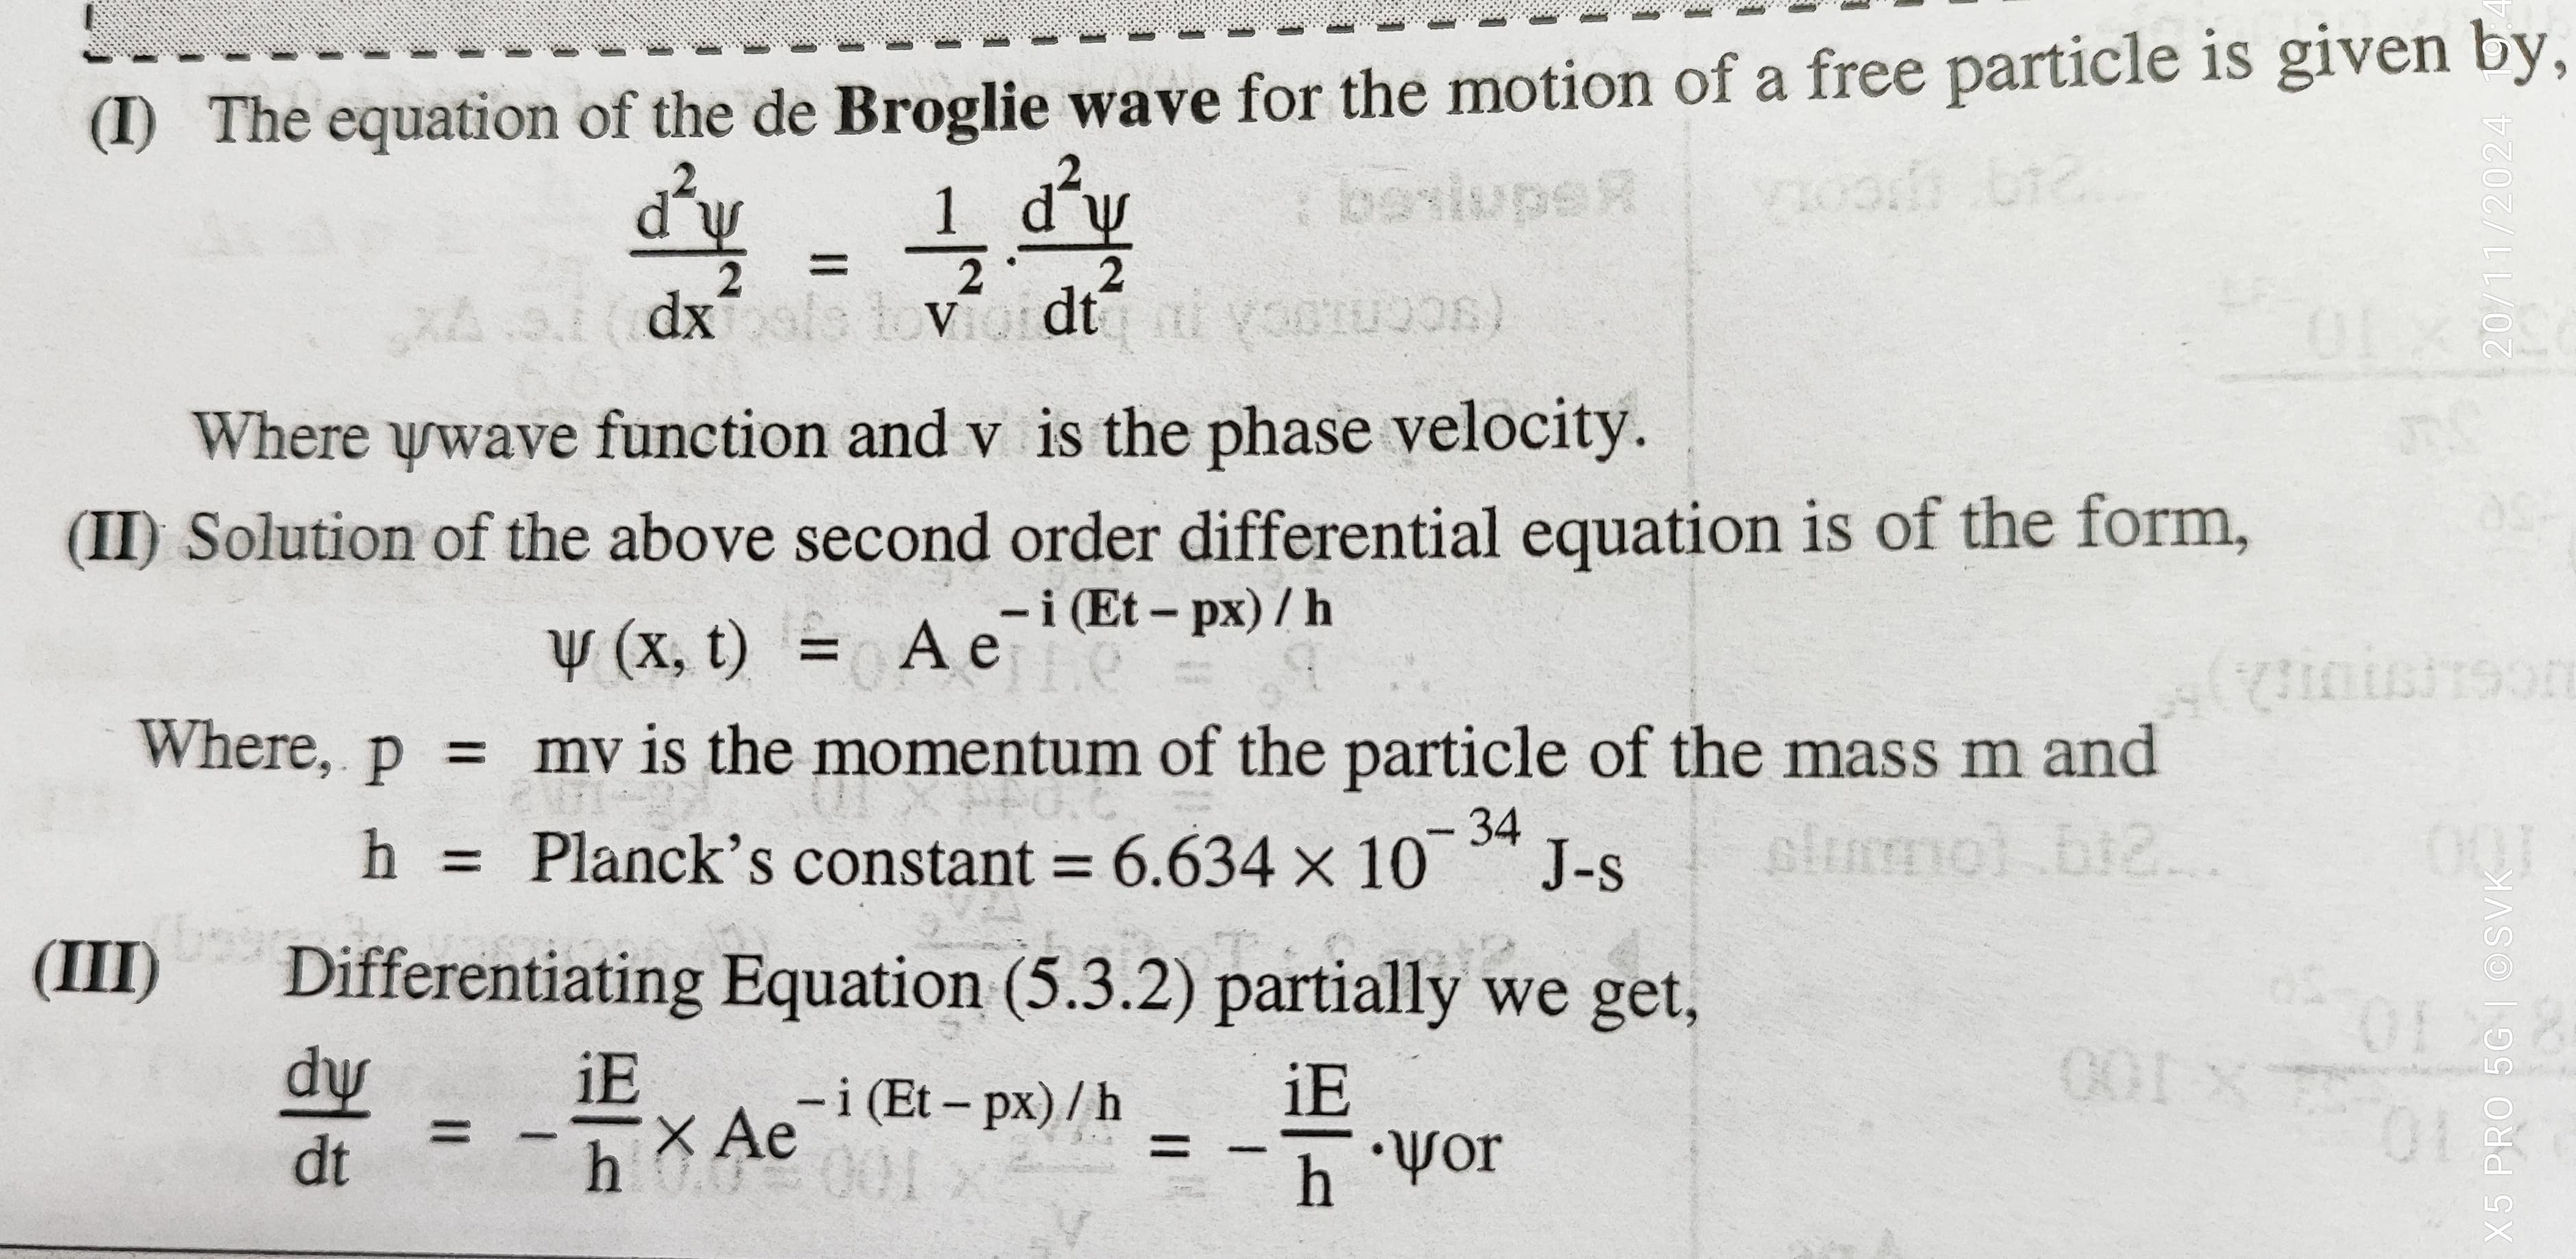
\includegraphics[scale=0.1]{Q12-1.jpeg}
	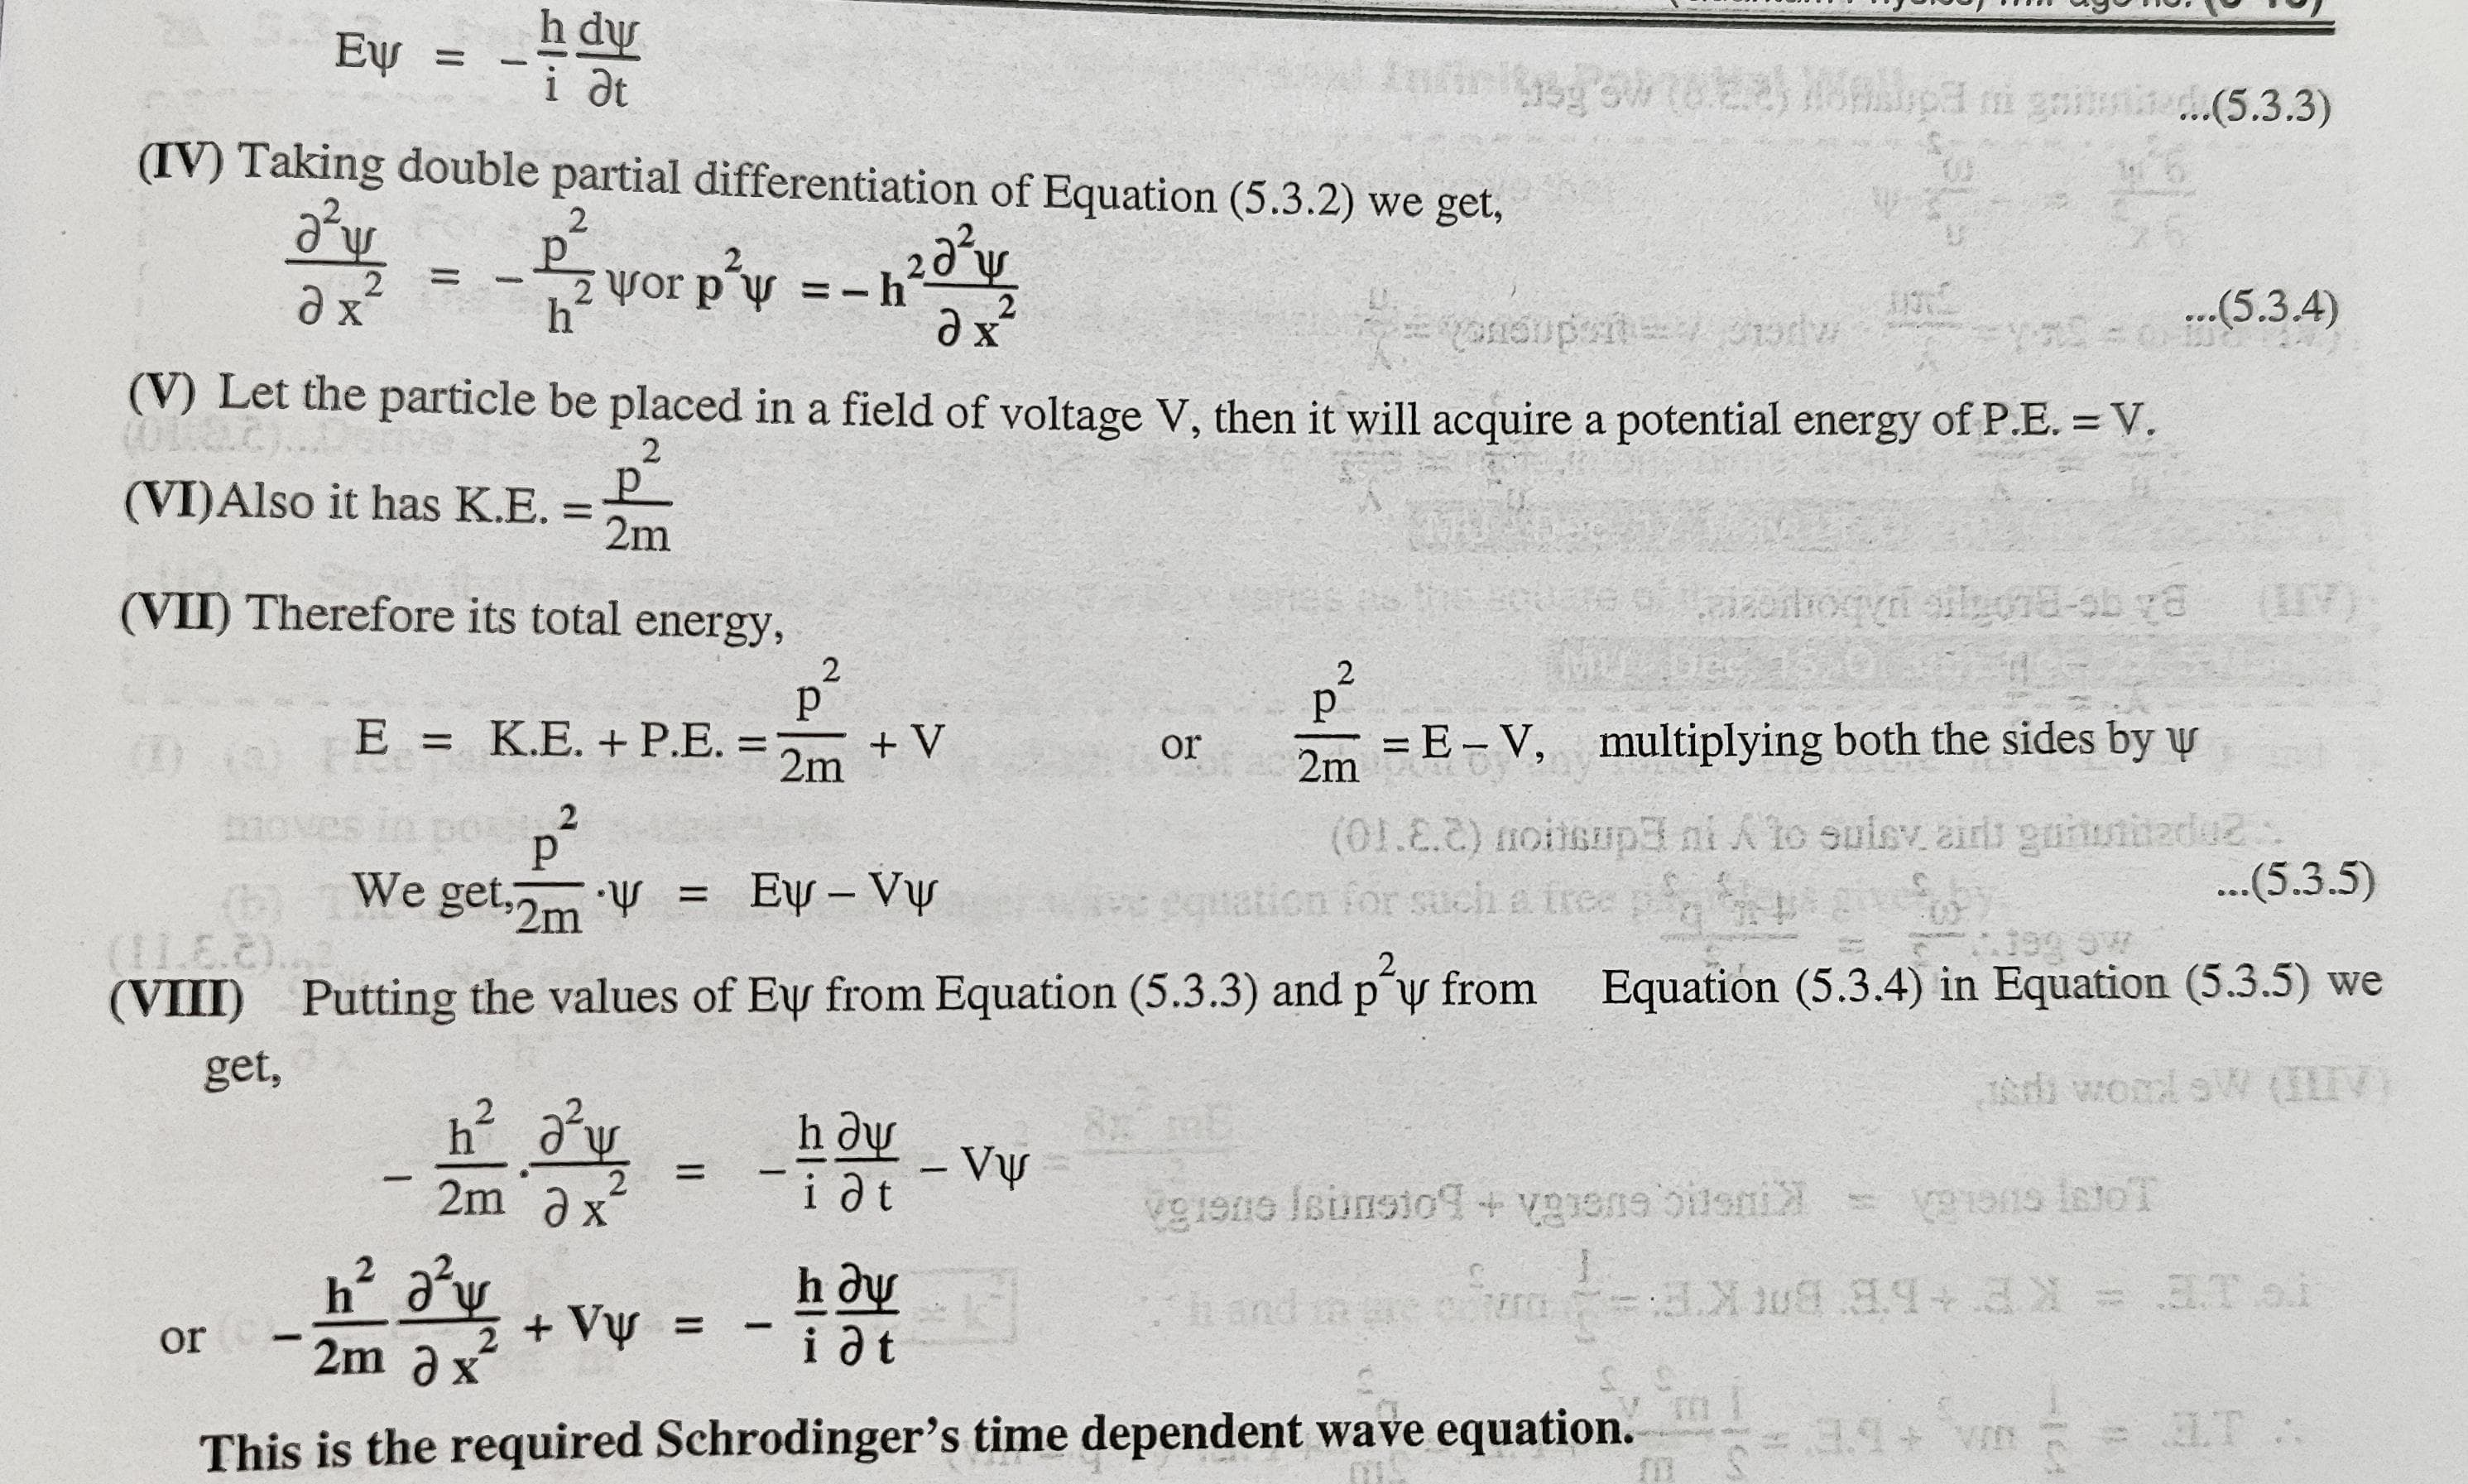
\includegraphics[scale=0.125]{Q12-2.jpeg}
\end{center}

\newpage

\question \textbf{Write the expression for Schrödinger's time dependent equation of matter waves and derive Schrodinger's time independent equation. \hfil [5 Marks] [May-2024]} 

\textbf{Ans:} State the Schrödinger's time dependent equation derived in Q.12 and then derive the following 
\begin{center}
	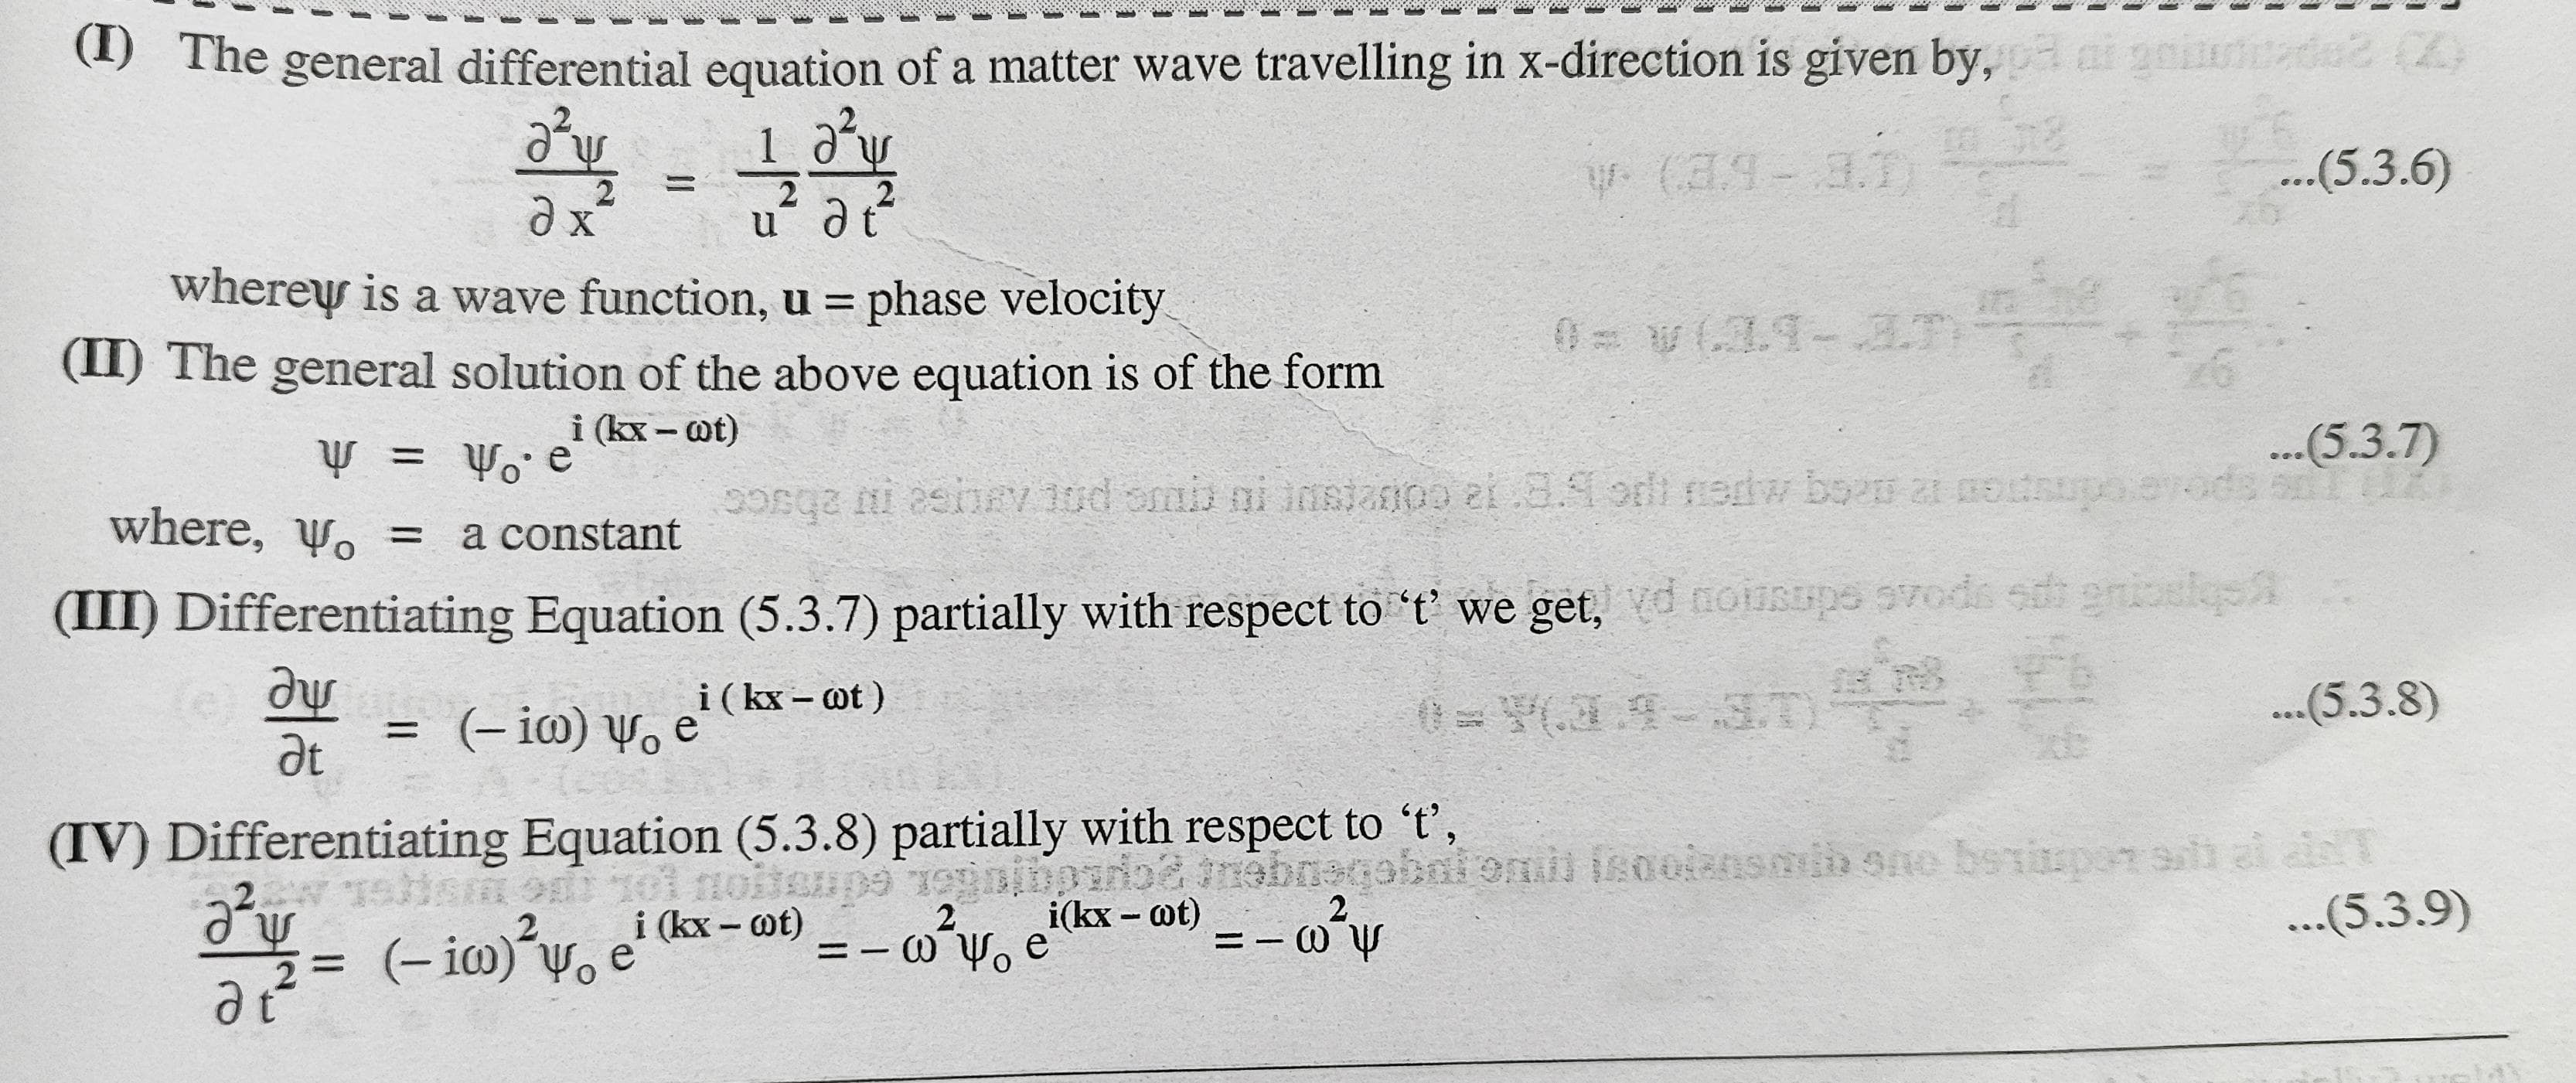
\includegraphics[scale=0.1]{Q13-1.jpeg}
	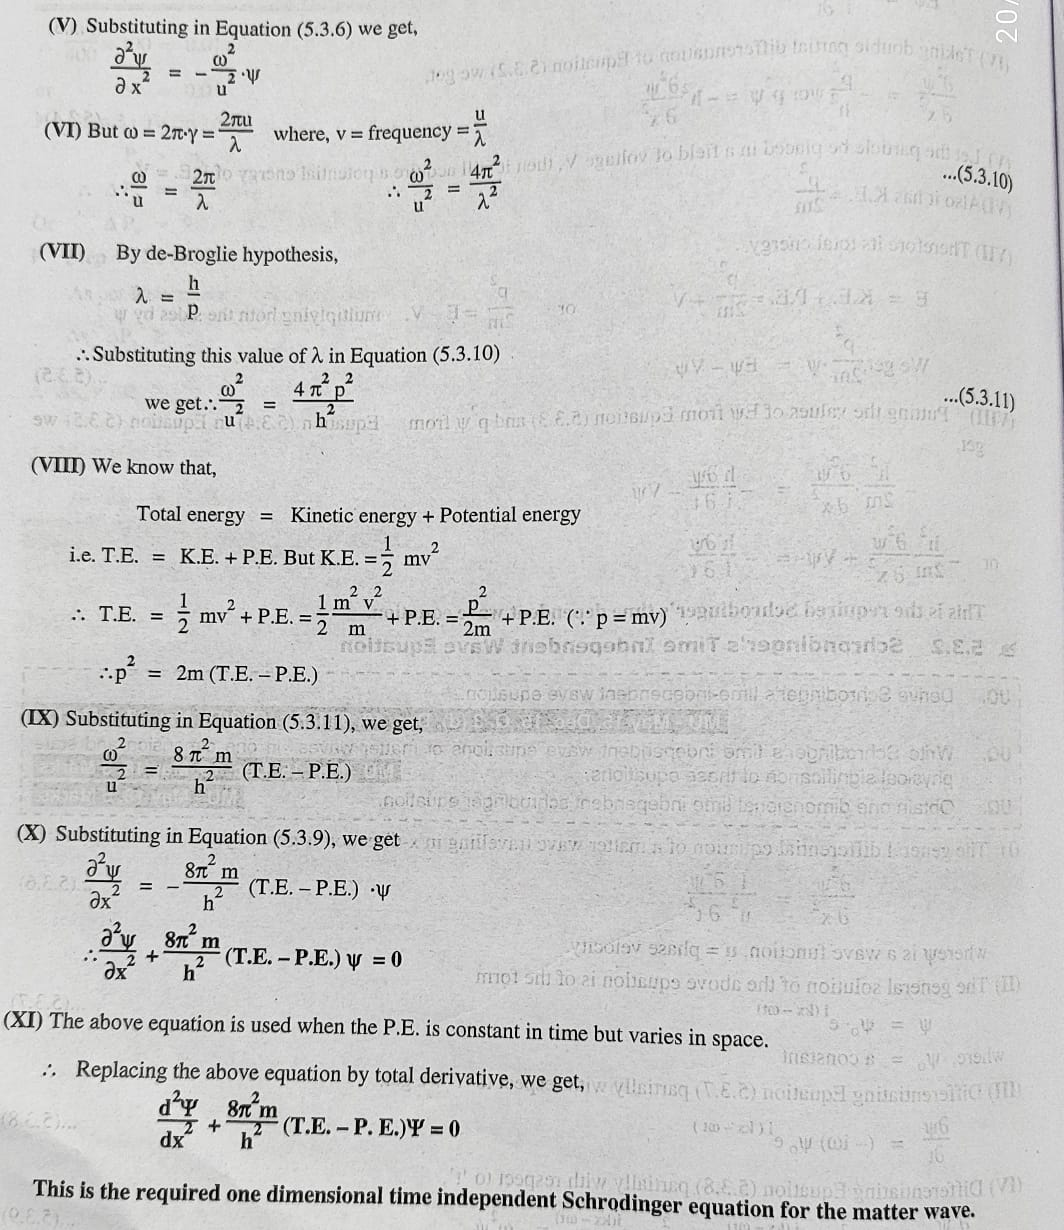
\includegraphics[scale=0.315]{Q13-2.jpeg}
\end{center}


\newpage

\begin{center} \textbf{ \Large Particle Enclosed in a Rigid Box} \end{center}

\question \textbf{Derive the expression for energy eigen values for free particle in one dimensional potential well. \hfil [4 Marks] [May-2022] 
\\ OR \\
Show that the energy of an electron in a one-dimensional deep potential well of infinite height varies as the square of the natural numbers.  \hfil [7Marks] [May-2022] }

\textbf{Ans:} 
\begin{center}
	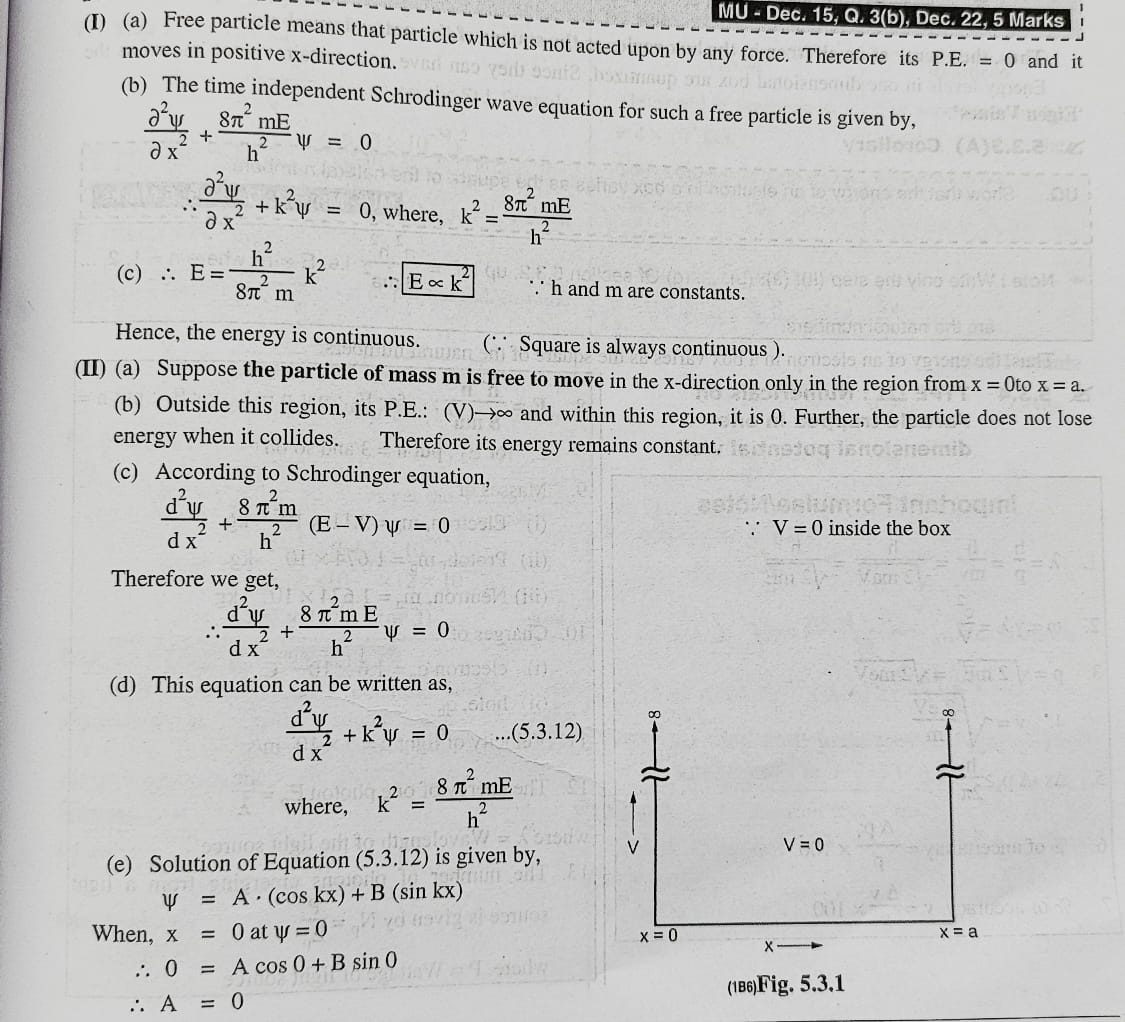
\includegraphics[scale=0.33]{Q14-1.jpeg}
	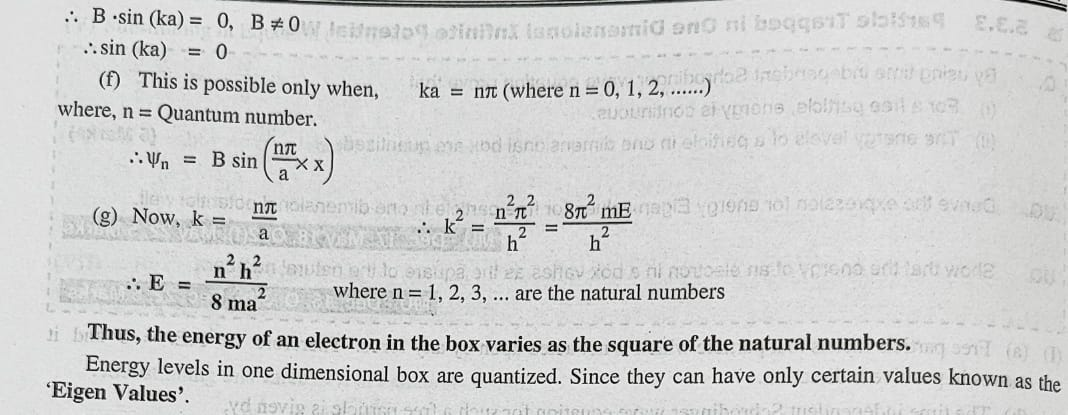
\includegraphics[scale=0.35]{Q14-2.jpeg}
\end{center}

\newpage
\question \textbf{The ground state energy of an electron in an infinite well is 5.6 x$10^{-3}$ eV. What will be the ground state energy if the width of the well is doubled?  \hfil[4 Marks] [May-2022] }

\textbf{Ans:} 
\begin{center}
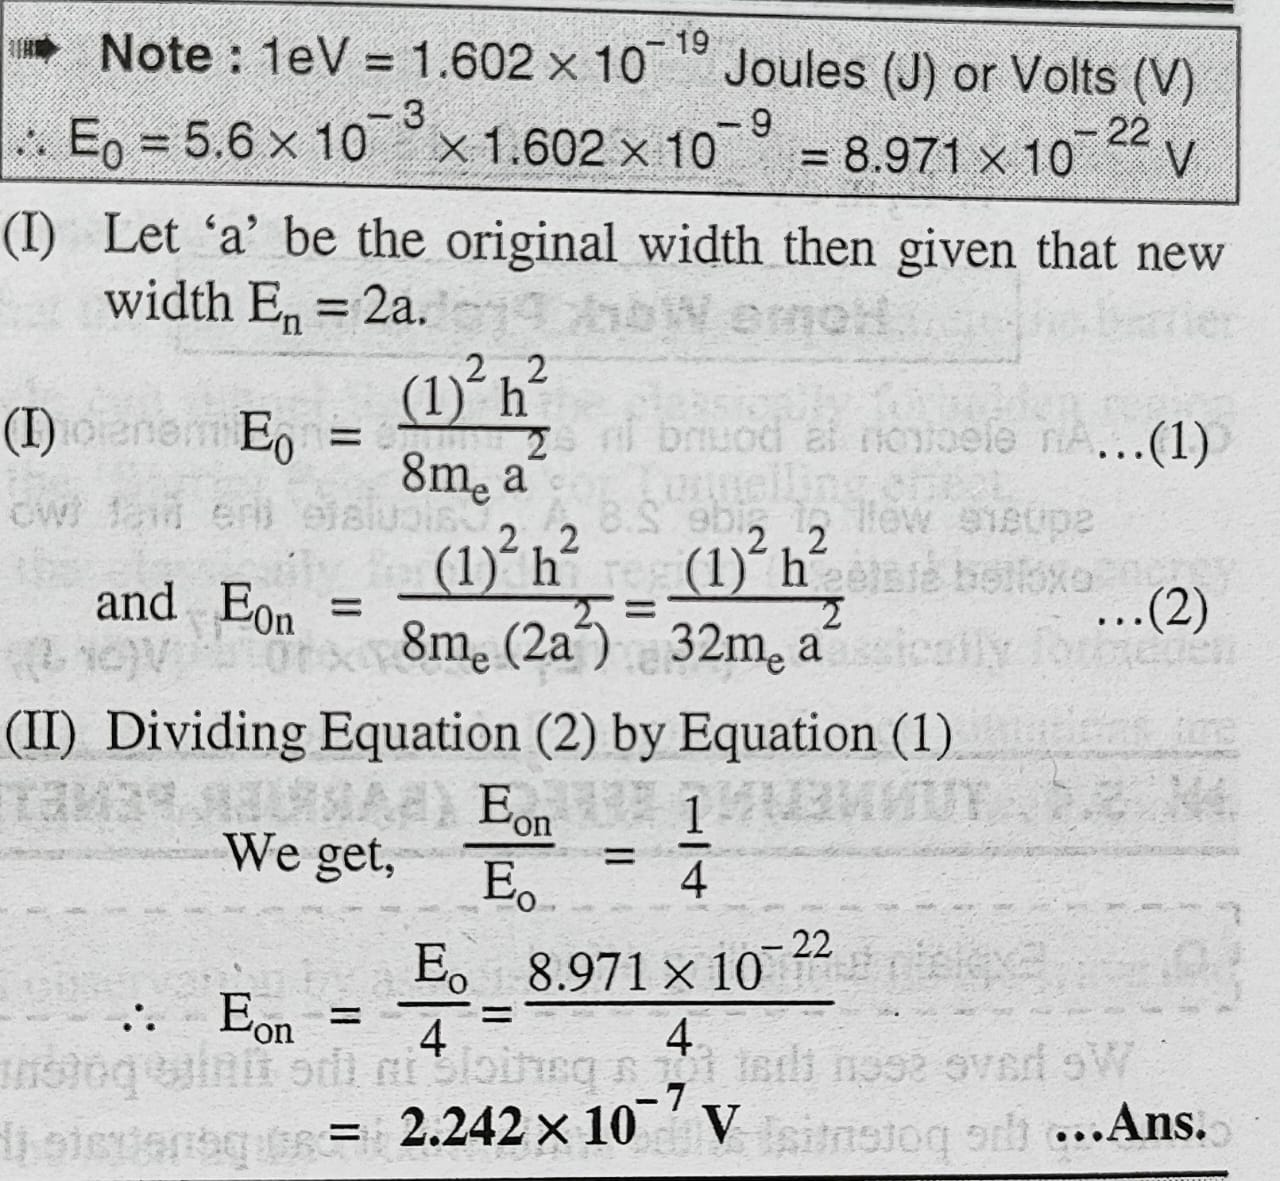
\includegraphics[scale=0.3]{Q15.jpeg}
\end{center}


\question \textbf{An electron is bound in a one-dimensional potential well of width 2 A° but of infinite height. Find its energy values in the ground state and in first excited state. \hfil [3 Marks] [Dec-2022] }

\textbf{Ans:} 
\begin{center}
	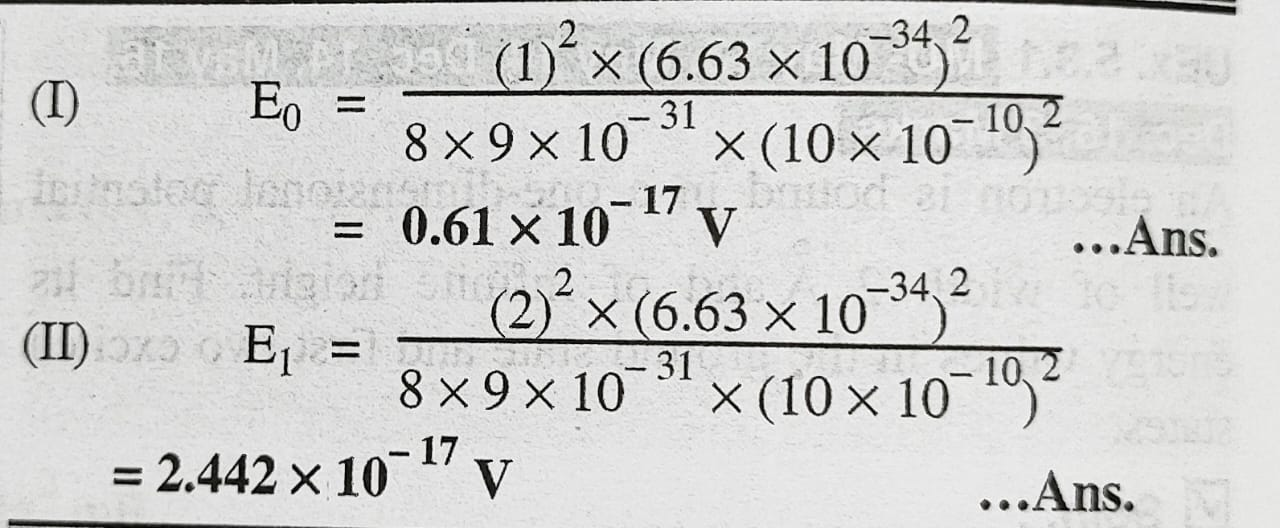
\includegraphics[scale=0.3]{Q16.jpeg}
\end{center}

\newpage
\question \textbf{The minimum energy possible for a particle trapped in a 1-d box is 3.2 x $10^{-18}$  J. What are the next 5 three energies in eV the particle can have? \hfil  [5 Marks] [May-2023] }

\textbf{Ans:} 
\begin{center}
	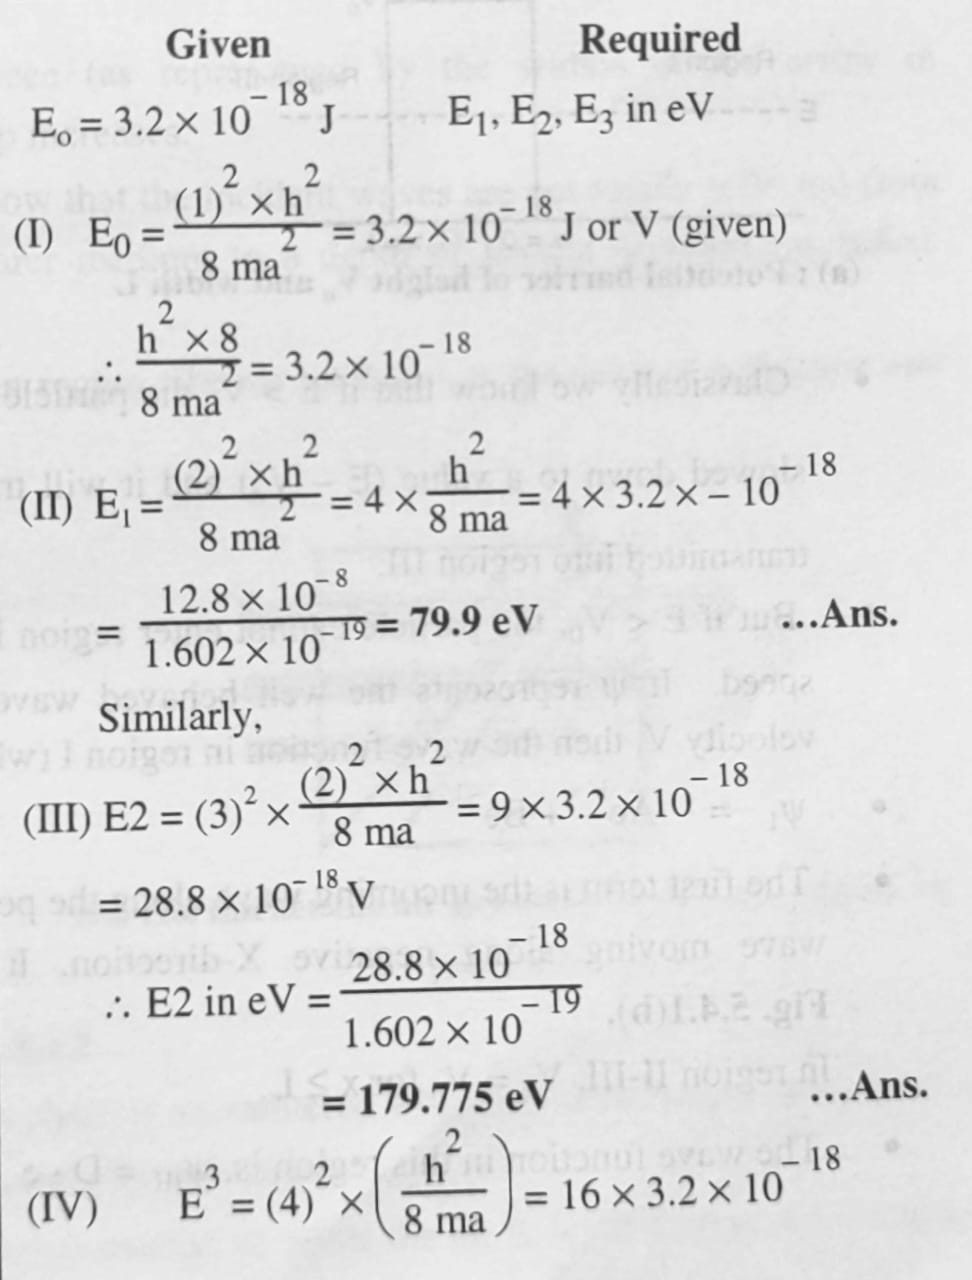
\includegraphics[scale=0.35]{Q17.jpeg}
\end{center}

Concert E3 in eV from Joules.
 
\question \textbf{An electron is bound in a one-dimensional potential well of width 5 $A^{\circ}$ but of infinite height. Find its energy values in the ground state and in first two excited states.  \hfil[5 Marks] [Dec-2023] }


\textbf{Ans:} Similar to above problem(s)


\end{questions}
	
\end{document}
